\documentclass{article}

\usepackage[utf8]{inputenc}
\usepackage{multirow}


\title{Smart Vacuum Robot}
\author{Harsh Aggarwal, Pranjal Aggarwal}
% \date{cs5190443@iitd.ac.in}
\date{}
 
\usepackage{natbib}
\usepackage{graphicx}
\usepackage[center]{caption}
\usepackage{amsmath}
\usepackage{amsfonts}
\usepackage{amssymb}
\usepackage{mathtools}
\usepackage[margin=1.2in]{geometry}
\usepackage{breqn}
\usepackage{siunitx}
\usepackage[ruled,vlined]{algorithm2e}
\usepackage[colorlinks=true,linkcolor=blue]{hyperref}
\usepackage{algorithmicx}
 

\DeclarePairedDelimiter{\ceil}{\lceil}{\rceil}

 
\begin{document}

\maketitle

\section{Introduction}

% Start of with something else, these points may come in doc but not here, as they are not directly relevant to our problem
With advent of modern technology, once a thing of future, is now becoming a common reality. However AI agents employed
in these systems have to face various challanges, as the cognitive abilities of AI is far less than that of humans. 
One such task is that of robot cleaning. The robot systems employed in this task have to sense the enviornment
and take decisions without harming the humans or other objects. At the same time these systems should be efficient enough to complete their task in
a limited time and also in limited amount of energy. In this report we study this problem of efficiency, and discuss various literature, which have tried to solve a problem similar to this.
We use them and build upon a new heuristic based approach.

\section{Problem Statement}

Suppose we have an indoor building with n rooms, which need to be cleaned. Each room may have different sizes
and floorplans, and different amount of dust in them. The task of the robot is to clean all the rooms in the building in a limited amount of time.
This limited time can be due to both limited battery or storage capacity of robot or urgency to complete the task(such as when public centrs are closed for only small duration in the whole day).

At the same the robot has to maximise the amount of cumulative amount of dust cleaned in all rooms, while providing a minimum in each of the room.
The problem can be modelled as a two stage problem:
\begin{itemize}
    \item In the first stage, we find the best path for the robot to reach all the rooms. This is a Travelling Salesman Problem we propose Steiner TSP Algorithm for this.
    \item In the second stage, we allot a certain time to each room based on their size, and the robot has to find a path which maximizes the dust cleaned, while at the same time is within the alloted budget of time.
\end{itemize}

Both of these stages can be modelled as a path finding in graph problem, where in first stage the pathway connecting rooms is equivalent to edges and the rooms as vertices.
For the second stage we divide a room into a grid of n*n cells, each either being occupied by an object, or having certain amount of dust. This grid can be considered as graph,
with the unoccupied cells as the vertices and the amount of dust in them as their vertex value. Since it will take slightly more time for robot to clean cells with larger dust amount,
the edge lengths will be dependent on the values of both the connected vertices:
\begin{equation}
    C_{i,j} = k + f(V_i,V_j)
\end{equation}
Where k is a constant value dependent on the speed of robot, and f is an arbitary function defined on the ordered values of two vertices.




\section{Related Work}

The problem at hand in stage 2 can be modelled as a variant of TSP  known as Profit-TSP. In this problem,
the Salesman has to maximise its profits however in a fixed finite amount of time. 
This has been shown to an NP-Hard Problem \cite{RAMESH1991151},\cite{apps2}. 
In literature various algorithms have been proposed, ranging from genetic algorithms to simple heuristic based algorithms. \cite{RAMESH1991151},\cite{rw1}.
In this report we will discuss in detail these works and also propose modifications to suit our needs in solving the aforementioned problem statement.

% TODO: Write about steiner if needed


\section{Steiner TSP solution}

The problem of starting from a point on the graph and returning to the same point after visiting a pre-determined fixed
set of points is called steiner TSP. A steiner TSP is just the extension of the TSP problem and can be converted to the
regular TSP problem very easily.

\subsection{Approach}

Consider a fully connected graph $G$ with vertex set $V$ and edge set $E$ such that $E \subseteq V \times V$. 
Given a set of vertices $U \subseteq V$ such that the starting vertex $v \in U$ and all vertices in $U$ must be visited
exactly once with the final vertex being $v$. \\

We can construct a subgraph $H \subseteq G$ such that $V_H = U$ and $E_H = V_H \times V_H$ i.e. a complete subgraph
comprising the vertex set $U$. We can define the edge length for an edge $e = (x,y) \in E_H,\ x,y \in V_H $ as the shortest
path length from $x$ to $y$ in $G$. i.e. $e(x,y) = d(x,y)$ where $e(x,y)$ is the length of edge from $x$ to $y$. \\

Executing TSP on the above subgraph $H$ will yield the corresponding solution to the steiner TSP problem on $G$. The TSP is 
solved using a Dynamic Programming approach. Let $dp(src, visited)$ indicate the shortest path length starting from $src$ to 
$v$, given that the set of already visited vertices is represented by the bit mask 
\footnote{
    If the number of vertices involved is $N$ the $visited$ argument is an integer in the range $[1, 2^N]$. The $i^{th}$ bit of
    the number $visited$ indicates whether the $i^{th}$ vertex is visited or not. To mark a vertex as visited we simply set the $i^{th}$
    bit of the number. It is a very efficient approach for encoding information in small constrainted problems and is popularly known as \textit{bit masking}.
}
$visited$. \\

To solve the DP we follow the steps below.
\begin{enumerate}
    \item Mark $src$ as visited by setting its bit in the $visited$ argument.
    \item For all the unvisited neighbors of $src$ calculate the sum of the edge length and the answer returned by the recursive call to $dp(neighbor, visited)$ which is the length of the shortest path from the neighbor to $v$ with the updated $visited$ bit mask.
    \item Calculate the minimum of all path lengths and store it as the optimal solution for this problem.
\end{enumerate}
Memoization of the results in an array of size $N \times 2^N$ ensures each subproblem is solved exactly once.

\begin{algorithm}[H]
    \SetAlgoLined
    visited $\gets$ visit(visited, src)\;
    optimalLength $\gets$ \verb|INT_MAX|\;
    \ForAll(){neighbor of src}{
        \If{!isVisited(visited, neighbor)}{
            pathLength $\gets$ edgeLength(src, neighbor) + dp(neighbor, visited)\;
            optimalLength $\gets$ min(optimalLength, pathLength)\;
        }
    }
    \Return{optimalLength};
    \caption{dp(src, visited)}
\end{algorithm}


\subsection{Proof of correctness}
The recursive $dp$ procedure can be proved easily using the principle of mathematical induction by inducting on $N$ (the number of vertices).

\textit{Base:}  The base case is for $n = 0$. The shortest path length is zero which matches with the algorithm output.\\

\textit{Induction Hypothesis: } For a given $n = n_0$, the procedure $dp(src, visited)$ returns the shortest path length from $src$ to $v$ after visiting all the vertices
exactly once and the initial visited vertices represented by the bitmask $visited$.\\

\textit{Induction step:} For a given $n = n_0 + 1$ the algorithm marks the $src$ vertex as visited and then recursively calls the $dp$ procedure
with the updated bitmask. Observe that setting a vertex as visited implies that no solution to the subproblems are allowes to visit the vertex.
But this is equivalent to just removing the vertex from the graph for the subproblems. This leads to a graph with $n - 1$ nodes for which the recursive calls 
are made. Now for $n - 1 = n_0$ vertices the Induction Hypothesis can be invoked to state that the shortest distance from a neighbor of $src$ to $v$ is specified
by the recursive call $dp(neighbor, updated\_visited)$ where $updated\_visited$ is the updated bitmask after visiting $src$. If the cost of the edge is added
then the total path length is determined and taking a minimum of all path lengths from the unvisited neighbors yields the shortes path from $src$ to $v$.
Thus for $n = n_0 + 1$ the Induction Hypothesis holds true.\\


Hence by \textbf{principle of mathematical induction} we have shown that the algorithm $dp(src, visited)$ returns the shortest path length from $src$ to $v$ with the current visited
state represented by the bitmask $visited$.

\subsection{Analysis}

The total number of subproblems is $(N*2^N)$. This is also the size of the memo that will be used during memoization for the DP solution.
Hence the \textbf{space complexity} of solution is $\Theta(N*2^N)$. Now each subproblem requires a linear amount of time since it involves a 
search through all the neighbors of the source vertex. Since there are at most $\Theta(N*2^N)$ subproblems the \textbf{time complexity} of the 
algorithm is $\Theta(N^2*2^N)$
\newpage
\subsection{Simulation}
The TSP algorithm was implemented and its simulation screenshot is shown below. The robot starts from a certain point and is given 
a set of 8 points (or doors) to visit in any order. The objective of the simulation is to show that the robot takes the path that minimizes the
total path length and hence is the most energy efficient path.\\

The number of doors reached so far are displayed on the bottom left of the simulation and the progress of simulation is indicated by the progress bar.
The path length covered so far is indicated to the right of the progress bar. The simulation helps visualize all features of a real world scenario and
can be used efficiently for analysis of various scenarios.
\begin{figure}[h!]
    \centering
    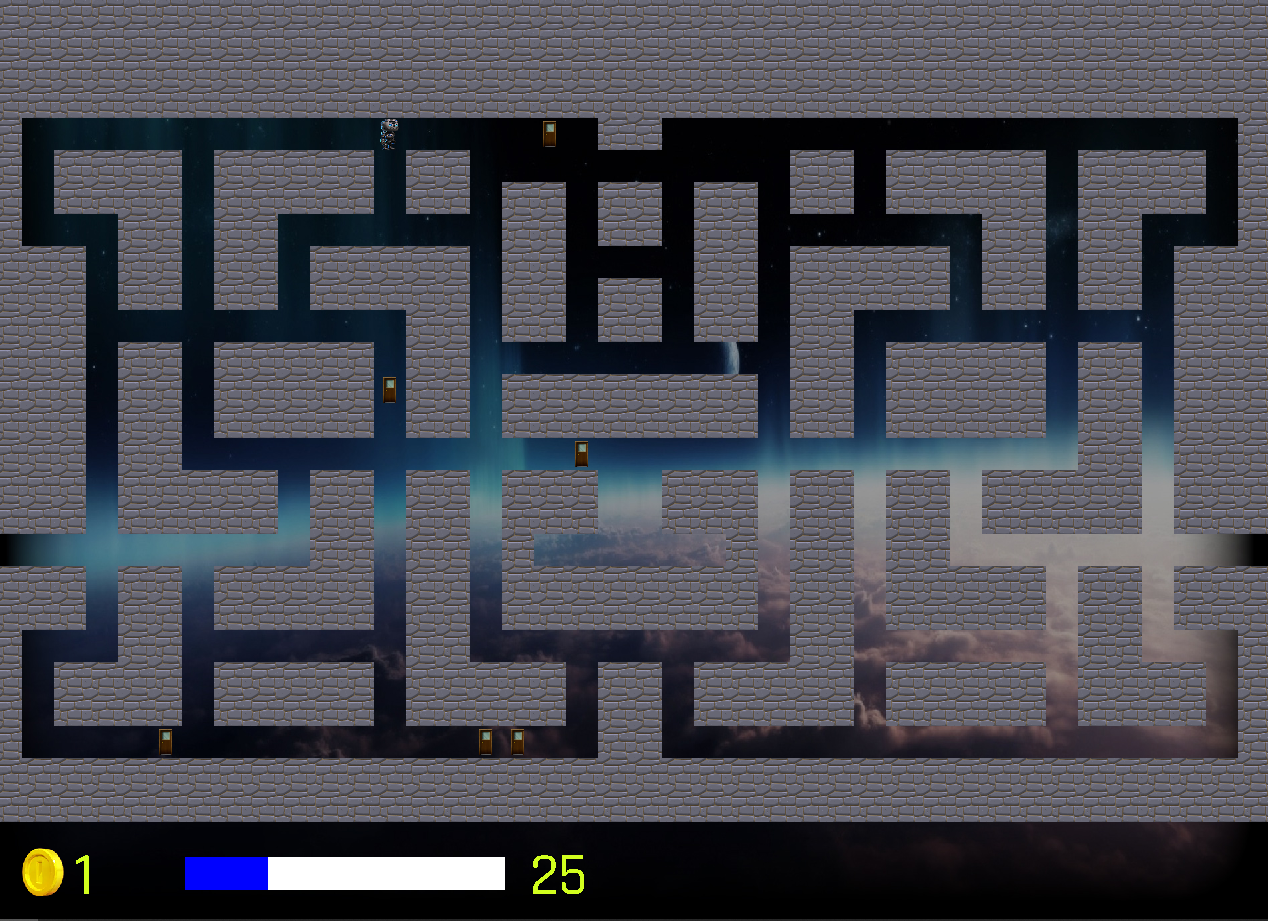
\includegraphics[width=\textwidth]{../sim.png}
    \caption{The robot is finding its path through the maze to reach the doors. It does so in such a manner that the total path length is minimized hence minimizing the energy consumption.}
\end{figure}

% \section{Computation and Results}

\newpage
\section{Solution: Time constrainted maximal coverage}

In this section we will discuss two possible heuristic solutions to our problem. The initial two stages 
are the same for both the approaches but they differ in the last step.

% \subsection{Centre of Gravity Based Algorithm}
% \cite{DEWILDE20131700} 
% Cite the Paper and write the content

% \subsection{Multi-Stage Algorithm}

% Check This
% While the previous algorithm requires an Euclidean cost function, in this algorithm we will model a genric enough cost function and solve the problem.

We divide the solution to the problem in multiple stages each performing a different operation. All these stages are iterated over for multiple rounds, till convergence criteria is not met.
We use 4 different hyperparameters whose values are determined empherically under some constraints.

\subsection{Stage I: Insertion Stage}

At the start of stage we assume that we have a path $\{L(i) : 0<i \leq k\}$, where k is the path length, and L(i) denotes the $i^{th}$ vertex in the path.
Since we have to start and end at the same position,
$L(1),L(2) = 1$.
We define two sets $\Psi$ and $\Omega$
, which contains the vertices in current path and and vertices not in current path respectively.
Now we first decide, a vertex to insert, lets call it $j$. Now we need to find a point in the path where we can insert the given vertex, and which gives maximum increase in profit while minimising the cost.
Then point of insertion can be found by solving the following Optimisation:

\begin{equation} \label{eq2}
    \Theta_{j} min_{i = 1,\dots,k} ( C_{V(i),j} + C_{j,V(i+1)} - C_{V(i),V(i-1)} )
\end{equation}
Where $\Theta_{j}$ is the calculated cost of given vertex for insertion.
Also note that in \refeq{eq2} we only need to iterate over only neigbours of vertex j, which in our case can be a maximum of 8, and therefore step 1 can be done in O(1) time.

Now we iterate over all the sutiable vertices for insertions, i.e and calculate the corresponding
$\Theta_{j}$. Now the best vertex is the one which give the maximum profit while with minimum cost i.e we try to take that vertex which has the highest profit to cost ratio.
Therefore we have to solve the following equation:

\begin{equation} \label{eq3}
    max_{j \in \Omega} \frac{P(j)}{C(j)} )
\end{equation}

However this would give high weightage to high density vertices therefore we add an additional hyperparameter $\lambda_1$ in \refeq{eq3},
and modify it as:

\begin{equation} \label{eq4}
    max_{j \in \Omega}  \frac{P(j)^{\lambda_{1}}}{C(j)}
\end{equation}

We hypothesize that $\lambda_{1} < 1$. This is due the fact that a minimum time is always required for robot to cross a cell, and thus by adding this additional hyperparameter,
we ensure that portions of small dust are not leftover.

We continue this process of insertion till the cost doesnt exceed $\lambda_{2,1} * \beta$, where $\lambda_{2,k}$ is another hyperparameter whose value varies in different rounds, and always increasing in subsequent rounds. 
If addition of any vertex increases the cost beyound alloted capacity, we omit it and move on to the next stage.

As we see that runtime complexity of this step is $O(n^2)$ in this case, wehere n is the final path length achieved after performin this stage. Note that its not $O(n^3)$ due to limited number of neighbours a vertex can have in the maze like structure we have used.


\subsection{Stage 2: k-Opt}
\label{kopt}
In this stage we apply the famous k-Opt Startegy \cite{opt1} \cite{opt2} increase the total profit while being in the budget. 
We start with applying 2-opt Optimisation, and if the final profit is more than $\{ \lambda_{3} , \lambda_{3} > 1 \}$ times the previous score, we move on to higher order k-opts. 
However if increase in budget is observed without satisfying the previous equation, we go back to stage-1 since further insertions may have scope for improvement. 
However if no increase in profit is improved, we move onto the next stage. The worst case complexity of this strategy on a complete graph is $O(n^2)$, however as in previous stage, since we have a maximum of 8 connexting edges from a vertex, the time complexity is just $O(n)$ for a single pass of this stage.

\subsection{Stage 3: Final stage}

There are two approaches discussed below for the last stage. The first approach deals with deleting vertices in the current path, whereas the second
approach uses a centre of gravity approach \cite{apps1} to modify the existing route.
\subsubsection{Deletion}

In this stage we try and delete vertices, that may not be useful for inclusion in path.
Let $S_{final}$ be the new profit after deleting a vertex $v$ from path $P$. Then we define a metric: 
\begin{equation}  \label{eq5}
    \xi (j)= \frac{S_{initial} - S_{final}}{P(j)}
\end{equation}
where j is the vertex removed from the path

Then we find the vertex $j \in P$ such that value of $\xi$ is minimised. What this means is that deletion of j gives the lowest per unit price loss.
After this step we check for the convergence criteria which terminates when the new overall profit $P_{ov}$ is atleast $\lambda_4$ times the overall profit in last round $P_{ov,last}$.
If the convergence criteria is not met we move back to stage 1 for further insertions and repeat the steps. 
Again the time complexity of this stage is $O(n)$ since we can delete only n points in the path, and deleteion of each point takes only $O(1)$ time

\subsubsection{Centre of Gravity}
Suppose now that node $i$ has coordinates $(x(i),y(i))$. In this step, we calculate
the center of gravity of $L$ as $g = (\bar{x} ,\bar{y})$, where
\begin{equation}  \label{eq6}
    \bar{x} =  \frac{\sum_{i \in L} P(i) x(i)}{\sum_{i \in L} P(i)}
\end{equation}
\begin{equation}  \label{eq6.2}
    \bar{y} =  \frac{\sum_{i \in L} P(i) y(i)}{\sum_{i \in L} P(i)}
\end{equation}

Let $a(i) = t(i,g)$ for $i = 1, 2, \ldots ,n$ i.e. the time taken to reach from $i$ to the centre of gravity $g$. Next a route including nodes $1$ and $n$ is formed as follows:
\begin{enumerate}
    \item Calculate the ratio $P(i)/a(i)\ \forall i$
    \item Add nodes to the route in decreasing order of this ratio using cheapest insertion, until no additional nodes can be added without exceeding the time constraint $T_{max}$.
    \item Use the \hyperref[kopt]{route improvement} step to make adjustments to the resulting
          route.
\end{enumerate}

We now have a route $L_1$. This route’s center of gravity gives rise to a repetition
of (1)-(3). The resulting route is denoted by $L_2$. This process is repeated until
a cycle develops, that is, route $L_p$ and $L_q$ are identical for some $q > p$. Finally,
we select the route that has the highest score among the routes
${L, L_1, L_2 , \ldots , L_q}$. 

This stage calculates the centre of gravity and the updated ratios at each iteration. This requires $\Theta(n)$ time in each iteration. Since there are $\Theta(n)$ iterations, the overall
time complexity of this stage is $\Theta(n^2)$. However we also repeat this stage $q$ times which would account for a higher complexity of $\Theta(qn^2)$. Typically,
$q$ is kept to be a static constant and is taken such that $q \le 10$. This ensures that the asymptotic analysis would yield a runninng time
given by $\Theta(n^2)$.
\subsection{Conclusion}

As we have shown the overall complexity of each stage is not more than $O(n^2)$ and therefore each round of algorithm is fast enough.
Also results in literature show that similar algorithms are able to achieve fast enough convergence, that they can be used in real time embedded systems, with minimum energy costs. \cite{RAMESH1991151}
Simulation data suggests that the robot was able to find a very good path in very less time, thus showing the effectiveness of this algorithm.

\subsection{Final Algorithm}

\begin{algorithm}[H]
    \SetAlgoLined
    \While{not converged}{
        1. Stage 1: Given a graph $G = (V,E)$ perform insertions based on \ref{eq4} till the cost doesnt exceed the specified value\;
        2. Stage 2: Apply k-opt strategy.
        \uIf{improvements are good enough}{
            Go to Stage 1 if \;
        }
        \Else{
            Move to Stage 3 \;
        }
        3. Stage 3: Perform Deletions of vertex in path in accordance with \ref{eq5}\;
    }
    \caption{Optimisation Algorithm}
\end{algorithm}



\section{Future Directions}

The algorithms discussed in this report were mostly tested on random mazes. While the results on them look promising, in future we would like to simulate the problem in real floorplans, and data.
Also this problem can be further extended by considering some more realistic settings, such as different speeds of robot in different terrain, getting more information about the dust, such as their weight, density etc, to create an more accurate timing model.

\section{Conclusion}


Overall we see that with the right heuristics the given NP-Hard problem can be solved with good accuracy, in a real-time. While we focussed on a single task, similar algorithms can be used 
in domains not discussed in this report. \cite{apps1},\cite{apps2} Also with advent of modern technologies with capabilities of replacing human beings at non-trivial taks, such algorithms will be the need of the hour as evident from our application to cleaning robots.
As robotics grows in the technological domain, more path routing and graph based algorithms would need to be implemented, the solutions of most of which are NP Hard. We have demonstrated that 
the appropriate heuristics can get us very close to the optimal solution as given by deterministic algorithms with exponential time complexities.

%TODO: Add additional things if needed


\clearpage
\bibliographystyle{plain}
\bibliography{sample}


\end{document}
